\subsection{Thiết kế cơ sở dữ liệu} \label{sec:erd_section}

Trong kiến trúc microservice, mỗi dịch vụ quản lý một cơ sở dữ liệu độc lập theo đúng ranh giới domain. Vì vậy, mô hình dữ liệu không sử dụng quá nhiều ràng buộc khóa ngoại như kiến trúc nguyên khối. Thay vào đó, các quan hệ giữa dữ liệu được thể hiện ở mức logic hoặc thông qua các cơ chế đồng bộ sự kiện giữa các dịch vụ.

Mô hình ERD ban đầu cho các service nghiệp vụ được nhóm xây dựng dựa trên kiến trúc nguyên khối tổng thể, sau đó được phân tách và nhóm các thực thể cùng quan hệ tương ứng vào các cơ sở dữ liệu riêng biệt dựa trên ranh giới của từng Microservice.

Bên cạnh các dịch vụ nghiệp vụ chính, hệ thống còn có orchestrator service, chịu trách nhiệm điều phối các quy trình phân tán theo mô hình saga. Do vai trò đặc thù của nó, ERD của orchestrator service không mô tả các thực thể nghiệp vụ như các service thương mại điện tử khác, mà tập trung vào việc lưu vết trạng thái của từng saga, từng bước xử lý và các sự kiện cần gửi đi thông qua Kafka. Các thực thể như saga\_instance, saga\_step, outbox\_event và compensation\_action được tổ chức nhằm hỗ trợ điều phối, theo dõi và khôi phục giao dịch phân tán một cách tin cậy.

Hình \ref{fig:erd_overview} chính là sơ đồ ERD mô tả các thực thể và quan hệ giữa chúng trong từng service của hệ thống. Sơ đồ ERD tổng quan mô tả các thực thể chính của từng domain trong hệ thống. Mỗi nhóm thực thể được tổ chức tách biệt theo chức năng. Các mối quan hệ giữa chúng chỉ mang tính chất tham chiếu logic nhằm mô tả dòng dữ liệu, không phải là ràng buộc vật lý trong cơ sở dữ liệu.

Sơ đồ mapping của các ERD sẽ được miêu tả cụ thể ở phần phụ lục

\begin{figure}[H]
    \centering
    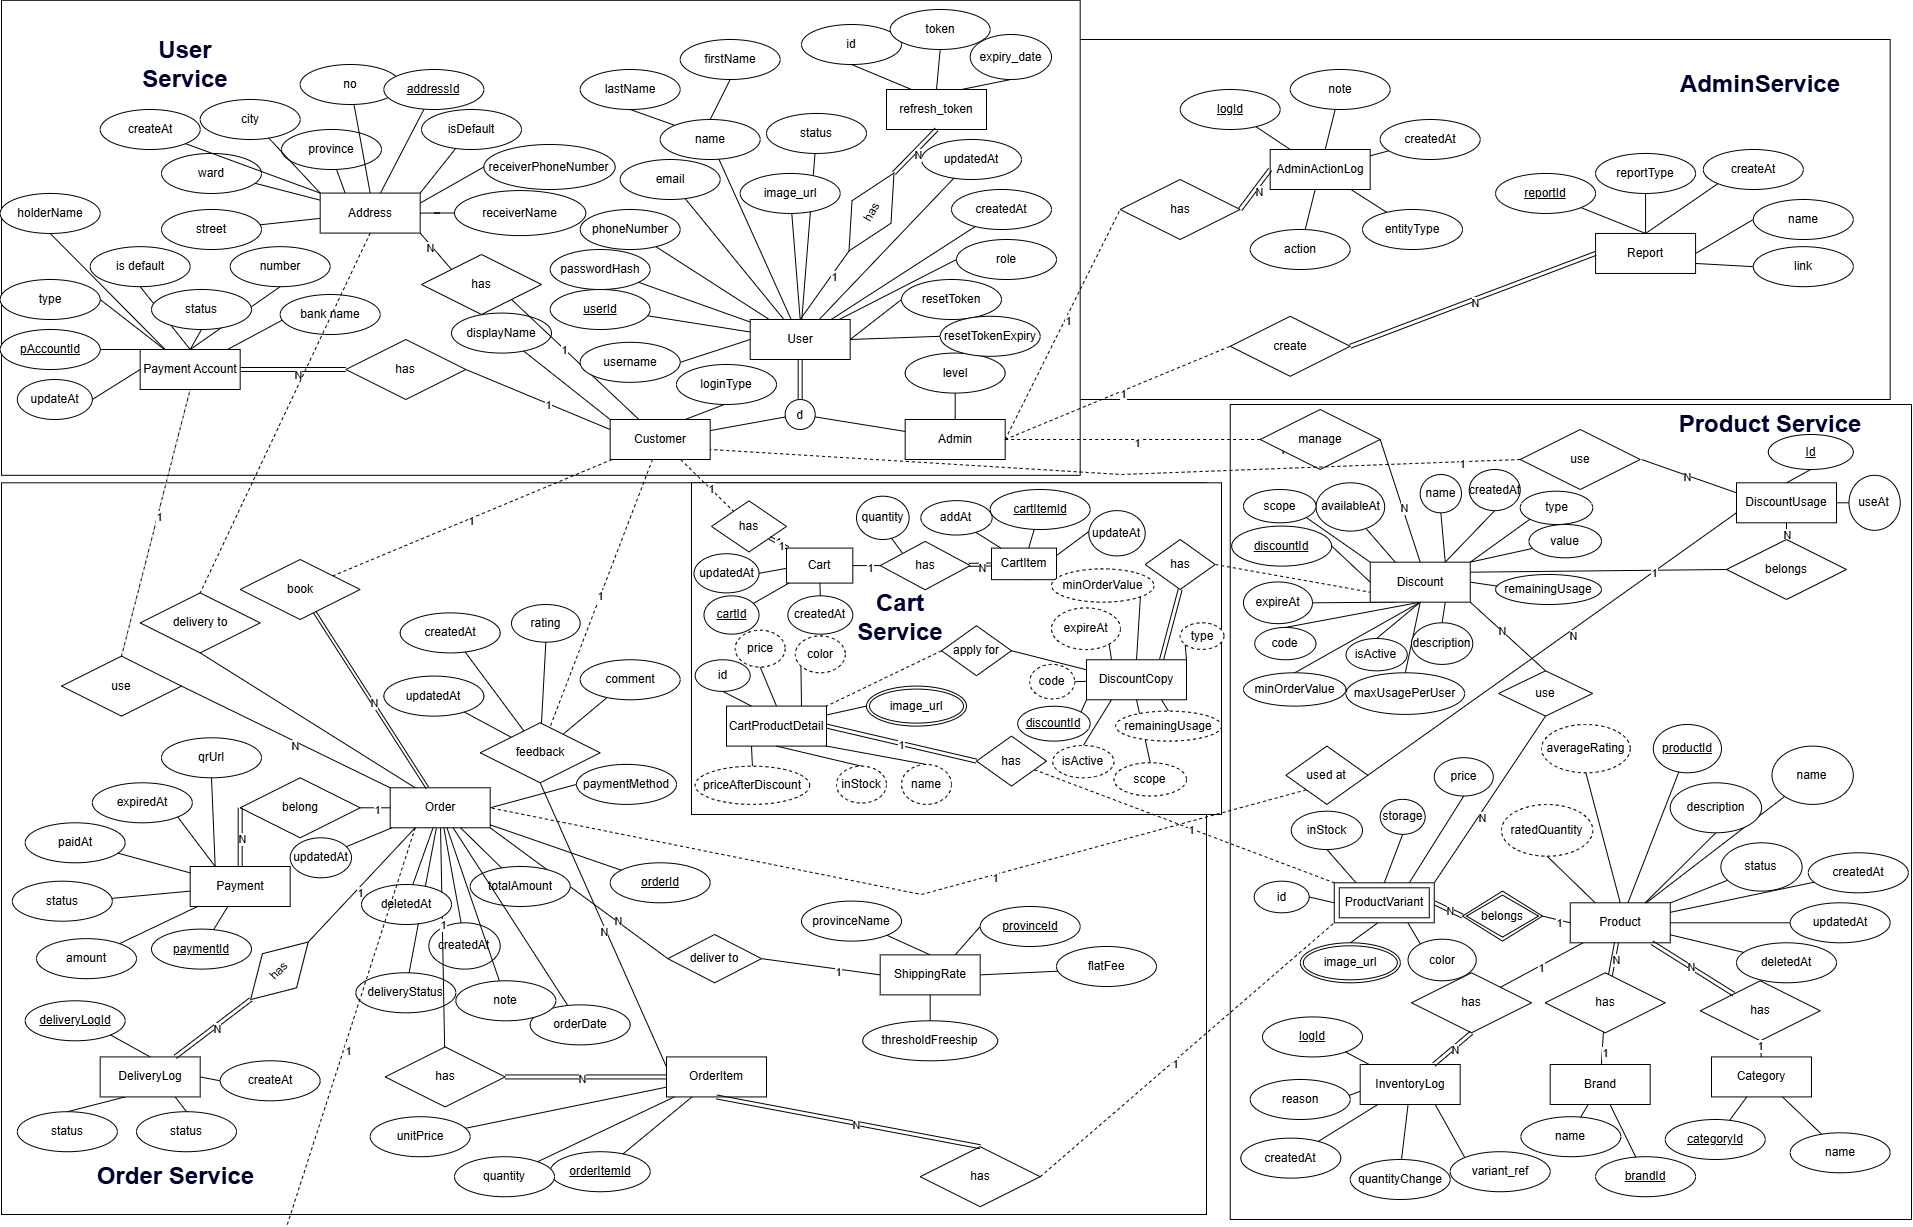
\includegraphics[width=0.9\linewidth]{images/chap6/erd/new_erd.png}
    \vspace{0.5cm}
    \caption{Sơ đồ ERD}
    \label{fig:erd_overview}
\end{figure}

Sơ đồ ERD của orchestrator service được trình bày bên dưới ở hình \ref{fig:erd_orches} nhằm làm rõ cách hệ thống triển khai Saga orchestration và cách các thành phần này phối hợp để đảm bảo tính nhất quán xuyên suốt nhiều microservice.

\begin{figure}[H]
    \centering
    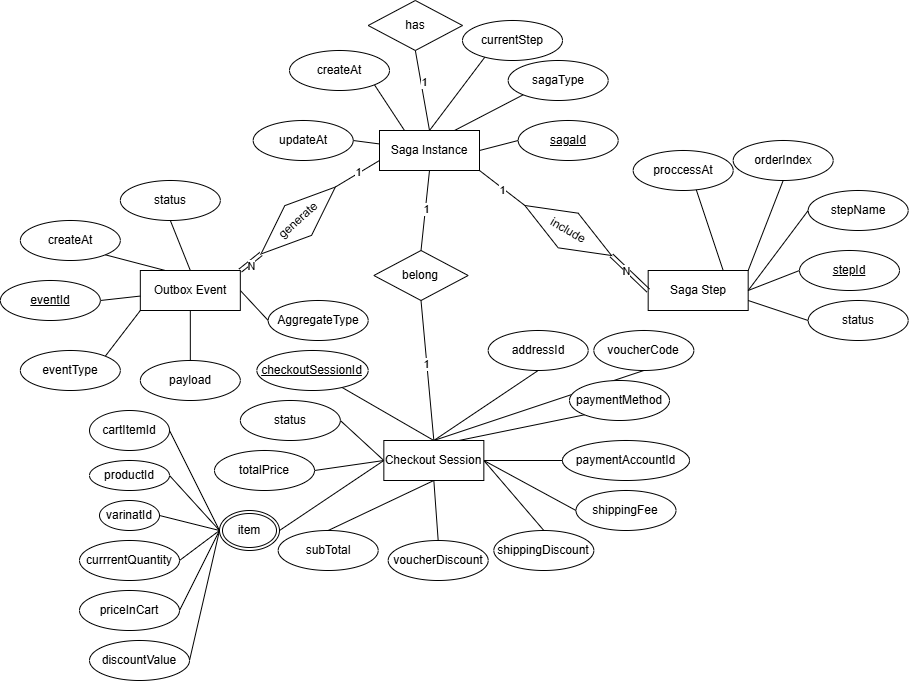
\includegraphics[width=0.9\linewidth]{images/chap6/erd/orchestration-erd.png}
    \vspace{0.5cm}
    \caption{ERD của orchestrator service}
    \label{fig:erd_orches}
\end{figure}

\subsubsection{ERD chi tiết cho user service}

Hình \ref{fig:user-service} mô tả cấu trúc dữ liệu của user service, đơn vị quản lý danh tính và thông tin giao dịch trong hệ thống.

User Service là domain chịu trách nhiệm quản lý danh tính và thông tin giao dịch cá nhân của tất cả người dùng trong hệ thống. Thực thể User đóng vai trò là cốt lõi, lưu trữ các thông tin định danh và có quan hệ disjoint để phân loại rõ ràng giữa Customer  và Admin, thể hiện sự phân quyền trong hệ thống. Để hỗ trợ bảo mật, thực thể Refresh Token có quan hệ 1:N với user giúp quản lý phiên đăng nhập lâu dài thông qua mã token và thời gian hết hạn.

Thực thể Customer mở rộng vai trò của người dùng thông thường và là trung tâm của các quan hệ giao dịch cá nhân. Mỗi Khách hàng có quan hệ 1:N với thực thể Address, cho phép lưu trữ nhiều địa chỉ giao hàng khác nhau. Đồng thời, Khách hàng cũng có quan hệ 1:N với thực thể Payment Account, quản lý các phương thức thanh toán đã liên kết.

\begin{figure}[H]
    \centering
    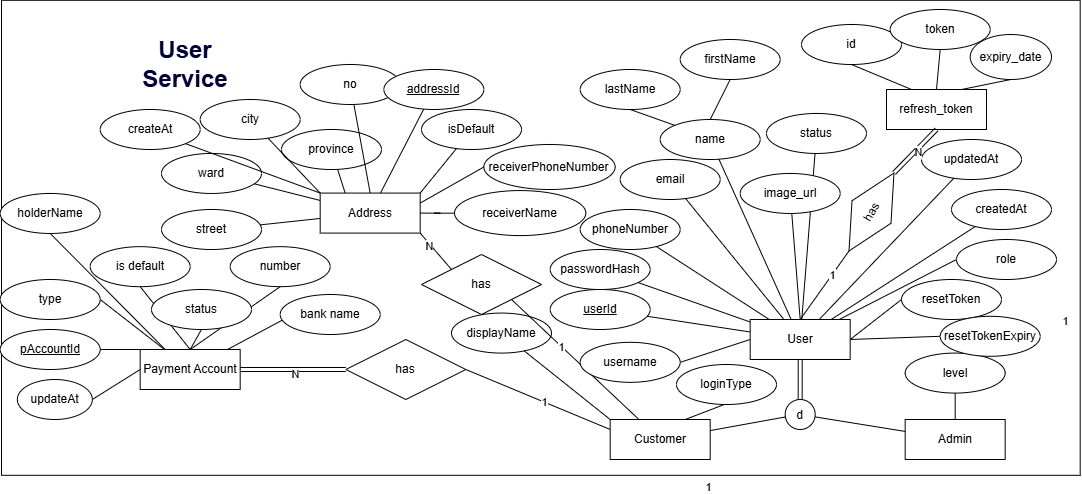
\includegraphics[width=1\linewidth]{images/chap6/erd/new-user-service-erd.png}
    \vspace{0.5cm}
    \caption{ERD chi tiêt cho user service}
    \label{fig:user-service}
\end{figure}

User service độc lập và chỉ quản lý các thực thể thuộc phạm vi người dùng. Mọi service khác trong kiến trúc Microservice, như Order Service, sẽ chỉ tham chiếu đến dữ liệu này bằng ID (ví dụ: userId, addressId) mà không cần lưu trữ lại thông tin chi tiết.

\subsubsection{ERD chi tiết cho product service}

Hình \ref{fig:product-service} mô tả cấu trúc dữ liệu của Product Service, domain cốt lõi quản lý danh mục sản phẩm, tồn kho và các chính sách khuyến mãi.

Thực thể Product đóng vai trò trung tâm, liên kết với Brand và Category qua các quan hệ N-1 để phân loại sản phẩm. Để tối ưu việc quản lý thuộc tính như màu sắc hay dung lượng, hệ thống sử dụng thực thể yếu ProductVariant có quan hệ N:1 với Product, giúp theo dõi chi tiết tồn kho và hình ảnh riêng biệt cho từng phiên bản. Mọi biến động hàng hóa đều được lưu vết qua thực thể InventoryLog.

\begin{figure}[H]
    \centering
    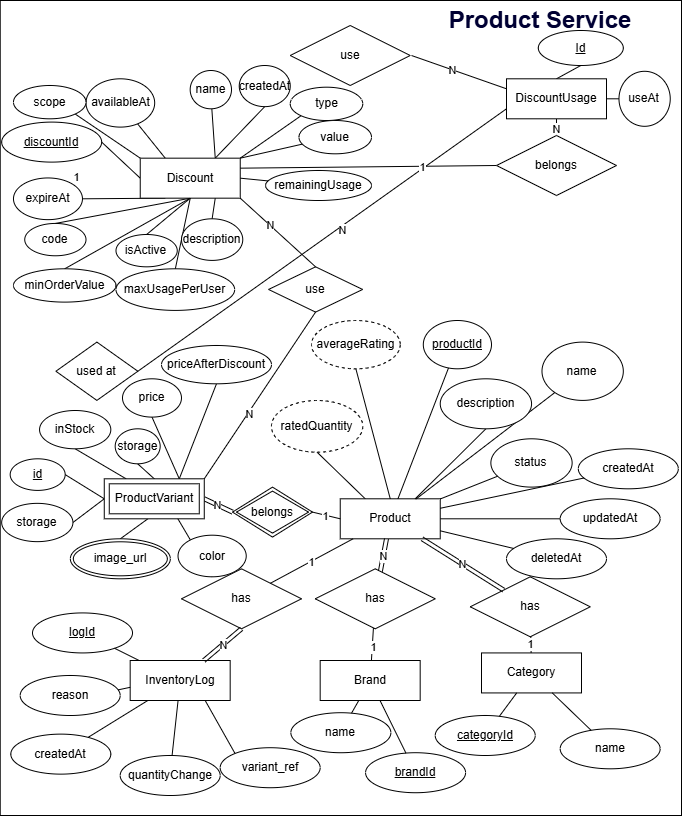
\includegraphics[width=0.6\linewidth]{images/chap6/erd/new-product-service.png}
    \vspace{0.5cm}
    \caption{ERD chi tiêt của product service}
    \label{fig:product-service}
\end{figure}

Hệ thống quản lý khuyến mãi thông qua thực thể Discount và DiscountUsage. Trong đó, DiscountUsage đóng vai trò quan trọng trong việc thiết lập các quan hệ logic liên dịch vụ: kết nối với thực thể Customer thuộc user service qua quan hệ use và thực thể Order thuộc order service qua quan hệ used at. Điều này giúp kiểm soát chặt chẽ việc áp dụng mã giảm giá cho từng khách hàng trên mỗi đơn hàng cụ thể.

\subsubsection{ERD chi tiết cho cart service}

Cart service được thiết kế tối giản nhằm quản lý trạng thái giỏ hàng tạm thời với hiệu suất cao. Thiết kế dữ liệu tập trung vào thực thể Cart, đại diện cho giỏ hàng duy nhất của mỗi khách hàng.

Thực thể Cart có quan hệ 1:1 với thực thể Customer thuộc user service thông qua quan hệ has để xác định chủ sở hữu. Thực thể CartItem lưu trữ danh sách mặt hàng khách hàng đã chọn kèm số lượng.  Để tối ưu tốc độ truy xuất và giảm tải cho việc gọi API liên dịch vụ, Cart Service lưu trữ các bản sao dữ liệu được đồng bộ từ product service thông qua Apache Kafka. Thay vì thiết lập quan hệ trực tiếp với thực thể Product ở dịch vụ khác, CartItem liên kết với thực thể bản sao CartProductDetail. Việc này nhằm đảm bảo thông tin sản phẩm luôn sẵn dùng ngay cả khi product service gặp sự cố, đồng thời loại bỏ độ trễ mạng khi phải truy vấn liên dịch vụ để hiển thị danh sách giỏ hàng.

\begin{itemize}
\item CartProductDetail: Bản sao tổng hợp từ Product và Product Variant giúp hiển thị giỏ hàng tức thời.
\item Discount: Bản sao thông tin khuyến mãi giúp tính toán tổng tiền trực tiếp tại dịch vụ mà không cần gọi API sang Product Service.
\end{itemize}

\begin{figure}[H]
    \centering
    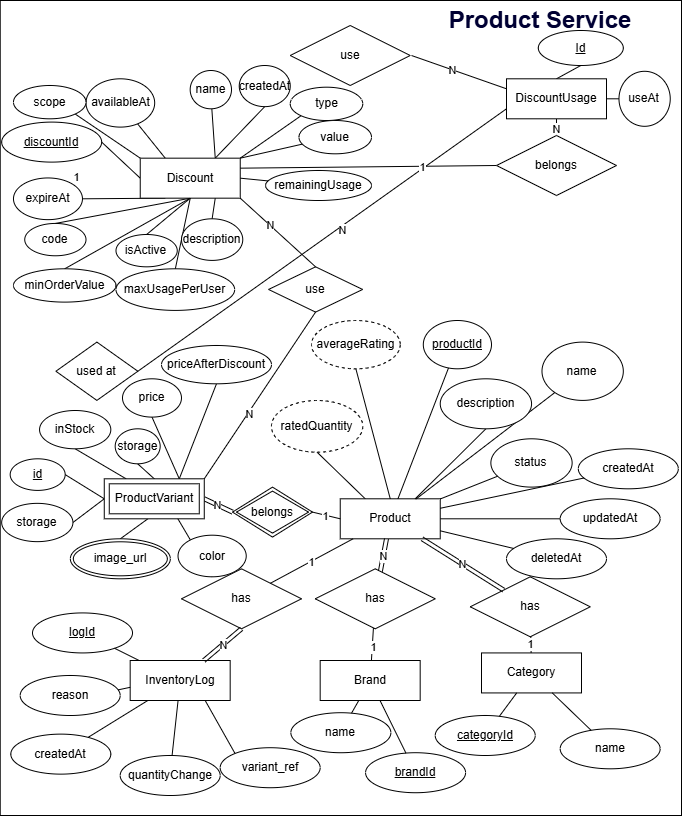
\includegraphics[width=0.6\linewidth]{images/chap6/erd/new-product-service.png}
    \vspace{0.5cm}
    \caption{ERD chi tiêt của cart service}
    \label{fig:cart-service}
\end{figure}

\subsubsection{ERD chi tiết cho order service}

Order Service chịu trách nhiệm quản lý toàn bộ vòng đời giao dịch từ đặt hàng, thanh toán đến hậu mãi. Thực thể Order đóng vai trò trung tâm, lưu trữ thông tin tổng quan và trạng thái đơn hàng.

Hệ thống quản lý chi tiết đơn hàng thông qua thực thể OrderItem có quan hệ 1:N với Order. Để theo dõi quá trình xử lý, mỗi đơn hàng liên kết với thực thể Payment qua quan hệ 1-1 để quản lý giao dịch tiền tệ và quan hệ 1-N với DeliveryLog nhằm ghi vết lịch sử vận chuyển. Ngoài ra, thực thể ShippingRate được sử dụng để xác định phí giao hàng dựa trên từng khu vực cụ thể.

Hình \ref{fig:order-service} minh họa các quan hệ ngoại lai logic để đảm bảo tính độc lập giữa các dịch vụ:

\begin{itemize}
\item book / feedback: Tham chiếu đến Customer ở user service để xác định chủ đơn hàng và người thực hiện đánh giá.
\item deliver to: Liên kết với Address ở user service và ShippingRate để xác định điểm đến và chi phí vận chuyển.
\item use: Tham chiếu đến Payment Account cũng ở user service để xác định nguồn thanh toán.
\item belong: Liên kết giữa Payment và Order để đối soát giao dịch.
\item has: Tham chiếu từ OrderItem đến Product thuộc product service để xác định mặt hàng.
\end{itemize}

\begin{figure}[H]
    \centering
    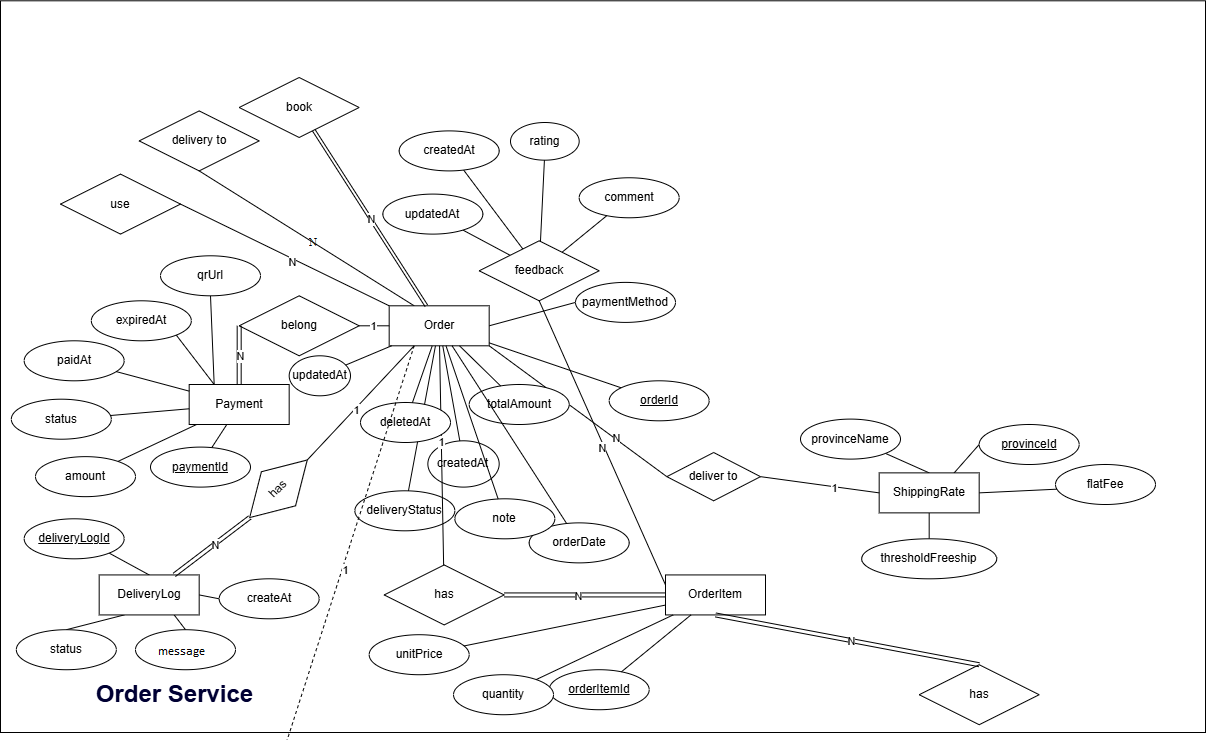
\includegraphics[width=1\linewidth]{images/chap6/erd/new-order-service.png}
    \vspace{0.5cm}
    \caption{ERD chi tiêt của order service}
    \label{fig:order-service}
\end{figure}

Việc chỉ lưu trữ các ID ngoại lai mà không có ràng buộc vật lý giúp order service duy trì tính độc lập cao, phù hợp với nguyên tắc thiết kế Database per Service trong kiến trúc Microservices.

\subsubsection{ERD chi tiết cho admin service}

Admin Service đóng vai trò là domain phụ trợ, chịu trách nhiệm duy trì tính minh bạch qua việc ghi vết hành động quản trị và quản lý các báo cáo hệ thống. Thực thể AdminActionLog đóng vai trò lưu trữ nhật ký thao tác chi tiết của quản trị viên, ghi nhận cụ thể loại hành động, thực thể bị tác động cùng các ghi chú liên quan để phục vụ mục đích kiểm soát tính minh bạch. Bên cạnh đó, thực thể Report chịu trách nhiệm quản lý danh mục các báo cáo thống kê đã được kết xuất. Thay vì lưu trữ trực tiếp dữ liệu thô gây tốn kém tài nguyên, thực thể này chỉ lưu giữ thông tin về loại báo cáo và đường dẫn liên kết đến tệp kết quả hoàn chỉnh.

Hình \ref{fig:admin-service} mô tả các mối liên kết ngoại lai nhằm duy trì tính nhất quán dữ liệu giữa các dịch vụ. Cụ thể, quan hệ has từ thực thể AdminActionLog và quan hệ create từ thực thể Report đều tham chiếu trực tiếp đến thực thể Admin thuộc User Service. Việc thiết lập các liên kết logic này giúp hệ thống định danh chính xác người chịu trách nhiệm cho từng thao tác quản trị cũng như xác định tác giả của các báo cáo thống kê được tạo lập.

\begin{figure}[H]
    \centering
    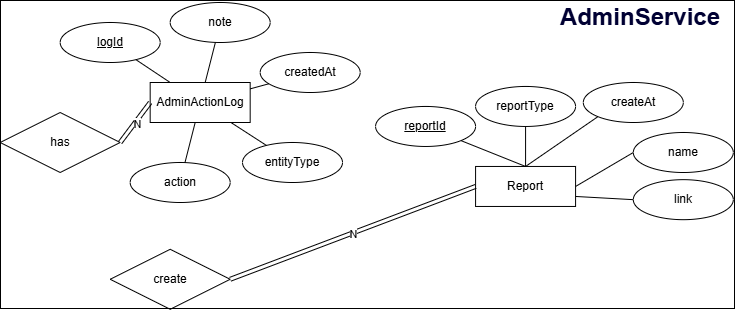
\includegraphics[width=0.9\linewidth]{images/chap6/erd/new-admin-service-erd.png}
    \vspace{0.5cm}
    \caption{ERD chi tiêt của admin service}
    \label{fig:admin-service}
\end{figure}


